\section{ĐƯỜNG TIỆM CẬN CỦA ĐỒ THỊ HÀM SỐ}
\subsection{LÝ THUYẾT CẦN NHỚ}
\subsubsection{Đường tiệm cận ngang (TCN):}
\begin{enumerate}[\iconMT]
	\item \indam{Định nghĩa:} Đường thẳng $y=m$ được gọi là một \inden{đường tiệm cận ngang} (hay \inden{tiệm cận ngang}) của đồ thị hàm số $y=f(x)$ nếu 
	$$\lim\limits_{x \rightarrow-\infty} f(x)=m \text{ hoặc }\lim\limits_{x \rightarrow+\infty} f(x)=m.$$
Đường thẳng $y=m$ là tiệm cận ngang của đồ thị hàm số $y=f(x)$ được minh hoạ như hình bên dưới
\begin{center}
	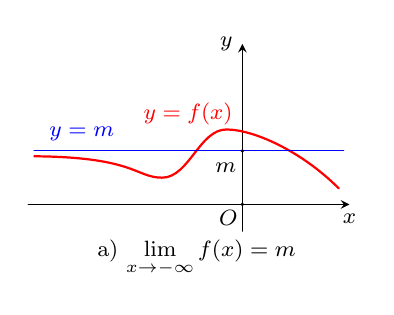
\begin{tikzpicture}[scale=0.68,>=stealth, font=\footnotesize, line join=round, line cap=round]
		\def\xmin{-4} \def\xmax{2}
		\def\ymin{-0.5} \def\ymax{3}
		%\draw[color=gray!50,dashed] (\xmin,\ymin) grid (\xmax,\ymax);
		\draw[->] (\xmin,0)--(\xmax,0) node [below]{$x$};
		\draw[->] (0,\ymin)--(0,\ymax) node [left]{$y$};
		\fill (0,0) circle (1pt) node[shift={(-135:2.5mm)}]{$O$};
		\node at (current bounding box.south) [below=-2pt] {a) $\lim\limits_{x \rightarrow-\infty} f(x)=m$};
		\clip (\xmin+0.1,\ymin+0.1) rectangle (\xmax-0.1,\ymax-0.1);
		\draw[red,thick,smooth,samples=300,domain=\xmin:\xmax]
		(-4,0.9)..controls +(0:2) and +(180:0.5)
		..(-1.5,0.5)..controls +(0:0.5) and +(180:0.5)
		..(-0.3,1.4)..controls +(0:0.5) and +(135:1)
		..(1.8,0.3);
		\draw [blue](\xmin,1)--(\xmax,1);
		\path[blue] (-3,1)node[above]{$y=m$};
		\path[red] (0,1.3)node[above left]{$y=f(x)$};
		\fill (0,1) circle (1pt) node[shift={(-135:3mm)}]{$m$};
	\end{tikzpicture}\hspace*{2cm}
	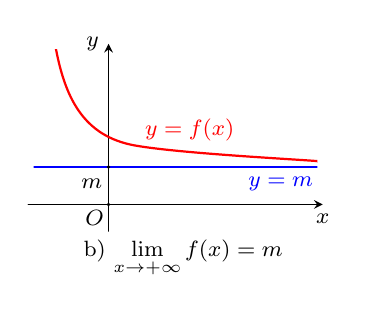
\begin{tikzpicture}[scale=0.68,>=stealth, font=\footnotesize, line join=round, line cap=round]
		\def\xmin{-1.5} \def\xmax{4}
		\def\ymin{-0.5} \def\ymax{3}
		%\draw[color=gray!50,dashed] (\xmin,\ymin) grid (\xmax,\ymax);
		\draw[->] (\xmin,0)--(\xmax,0) node [below]{$x$};
		\draw[->] (0,\ymin)--(0,\ymax) node [left]{$y$};
		\fill (0,0) circle (1pt) node[shift={(-135:2.5mm)}]{$O$};
		\node at (current bounding box.south) [below=-2pt] {b) $\lim\limits_{x \rightarrow+\infty} f(x)=m$};
		\clip (\xmin+0.1,\ymin+0.1) rectangle (\xmax-0.1,\ymax-0.1);
		\draw[red,thick,smooth,samples=300,domain=\xmin:\xmax]
		(-1,3)..controls +(-80:1) and +(170:1)
		..(0.5,1.1)..controls +(170:-1) and +(180:-0.5)
		..(3.9,0.8);
		\draw [blue](\xmin,0.7)--(\xmax,0.7);
		\path[blue] (4,0.7)node[below left]{$y=m$};
		\path[red] (0.5,1)node[above right]{$y=f(x)$};
		\fill (0,0.7) circle (1pt) node[shift={(-135:3mm)}]{$m$};
	\end{tikzpicture}
\end{center}	
	\item \indam{Các bước tìm TCN:}
	\begin{boxdn}
		\begin{itemize}
			\item [\ding{172}] Tính $\lim \limits_{x \to +\infty} f(x)$ và $\lim \limits_{x \to -\infty} f(x)$.
			\item [\ding{173}] Xem ở "vị trí" nào ra kết quả hữu hạn thì ta kết luận có tiệm cận ngang ở "vị trí" đó.
		\end{itemize}
	\end{boxdn}
\end{enumerate}
\subsubsection{Đường tiệm cận đứng (TCĐ)}
\begin{enumerate}[\iconMT]
	\item \indam{Định nghĩa:}	Đường thẳng $x=a$ được gọi là một \inden{đường tiệm cận đứng} (hay \inden{tiệm cận đứng}) của đồ thị hàm số $y=f(x)$ nếu ít nhất một trong các điều kiện sau thoả mãn:		
	$$
	\lim\limits_{x \rightarrow a^{-}} f(x)=+\infty,\,\, \lim\limits_{x \rightarrow a^{+}} f(x)=+\infty,\,\, \lim\limits_{x \rightarrow a^{-}} f(x)=-\infty,\,\, \lim\limits_{x \rightarrow a^{+}} f(x)=-\infty \text {. }
	$$
		Đường thẳng $x=a$ là tiệm cận đứng của đồ thị hàm số $y=f(x)$ được minh hoạ như hình bên dưới.
		\begin{center}
			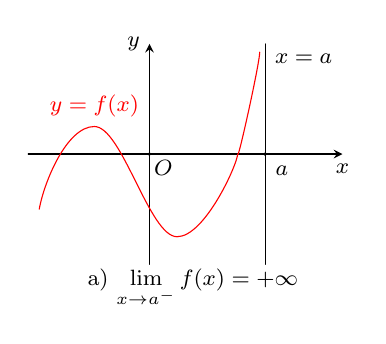
\begin{tikzpicture}[scale=.7,>=stealth, font=\footnotesize, line join=round, line cap=round]
				%Hình a
				\def\xmin{-2.2} \def\xmax{3.5}
				\def\ymin{-2} \def\ymax{2} 
				%\draw[color=gray!50,dashed] (\xmin,\ymin) grid (\xmax,\ymax); 
				\draw[->] (\xmin,0)--(\xmax,0) node [below]{$x$};
				\draw[->] (0,\ymin)--(0,\ymax) node [left]{$y$};
				\fill (0,0) circle (1pt) node[shift={(-45:2.5mm)}]{$O$};
				\draw (2.1,\ymin)--(2.1,\ymax)node[below right]{$x=a$};
				\fill (2.1,0) circle (1pt) node[shift={(-45:3mm)}]{$a$};
				%\clip (\xmin+0.1,\ymin+0.1) rectangle (\xmax-0.1,\ymax-0.1);
				\draw[red] (-2,-1)..controls +(80:0.5) and +(0:-.5)..(-1,0.5)node[above]{$y=f(x)$}
				..controls +(0:0.5) and +(180:0.5)..(0.5,-1.5)
				..controls +(0:0.5) and +(87:-0.2)..(1.6,0)
				..controls +(87:-.2) and +(90:-0.2)
				..(2,1.85);
				\node at (current bounding box.south) [below=-2pt] {a) $\lim\limits_{x \rightarrow a^{-}} f(x)=+\infty$};
			\end{tikzpicture}
			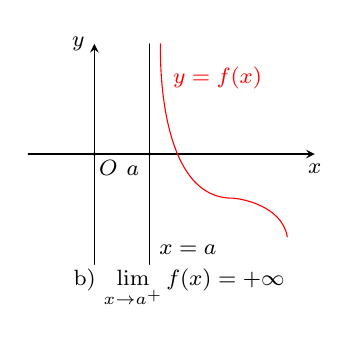
\begin{tikzpicture}[scale=.7,>=stealth, font=\footnotesize, line join=round, line cap=round]
				%Hình b
				\def\xmin{-1.2} \def\xmax{4}
				\def\ymin{-2} \def\ymax{2} 
				%\draw[color=gray!50,dashed] (\xmin,\ymin) grid (\xmax,\ymax); 
				\draw[->] (\xmin,0)--(\xmax,0) node [below]{$x$};
				\draw[->] (0,\ymin)--(0,\ymax) node [left]{$y$};
				\fill (0,0) circle (1pt) node[shift={(-45:2.5mm)}]{$O$};
				\draw (1,\ymin)node[above right]{$x=a$}--(1,\ymax);
				\fill (1,0) circle (1pt) node[shift={(-135:3mm)}]{$a$};
				\path[red] (1.25,1)node[above right]{$y=f(x)$};
				%\clip (\xmin+0.1,\ymin+0.1) rectangle (\xmax-0.1,\ymax-0.1);
				\draw[red] (1.2,2)..controls +(80:0) and +(0:-1.4)..(2.5,-0.8)
				..controls +(0:0.1) and +(-80:-0.6)
				..(3.5,-1.5);
				\node at (current bounding box.south) [below=-2pt] {b) $\lim\limits_{x \rightarrow a^{+}} f(x)=+\infty$};		
			\end{tikzpicture}
			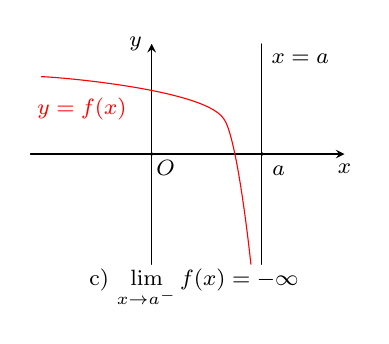
\begin{tikzpicture}[scale=.7,>=stealth, font=\footnotesize, line join=round, line cap=round]
				%Hình c
				\def\xmin{-2.2} \def\xmax{3.5}
				\def\ymin{-2} \def\ymax{2} 
				%\draw[color=gray!50,dashed] (\xmin,\ymin) grid (\xmax,\ymax); 
				\draw[->] (\xmin,0)--(\xmax,0) node [below]{$x$};
				\draw[->] (0,\ymin)--(0,\ymax) node [left]{$y$};
				\fill (0,0) circle (1pt) node[shift={(-45:2.5mm)}]{$O$};
				\draw (2,\ymin)--(2,\ymax)node[below right]{$x=a$};
				\fill (2,0) circle (1pt) node[shift={(-45:3mm)}]{$a$};
				\path[red] (-2.25,1.2)node[below right]{$y=f(x)$};
				%\clip (\xmin+0.1,\ymin+0.1) rectangle (\xmax-0.1,\ymax-0.1);
				\draw[red] (-2,1.4)..controls +(-10:-0.2) and +(-55:-.7)
				..(1.3,0.65)..controls +(-50:0.4) and +(-90:0)
				..(1.8,-2)
				;
				\node at (current bounding box.south) [below=-2pt] {c) $\lim\limits_{x \rightarrow a^{-}} f(x)=-\infty$};		
			\end{tikzpicture}
			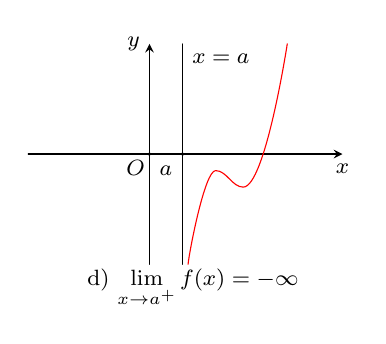
\begin{tikzpicture}[scale=.7,>=stealth, font=\footnotesize, line join=round, line cap=round]
				%Hình d
				\def\xmin{-2.2} \def\xmax{3.5}
				\def\ymin{-2} \def\ymax{2} 
				%\draw[color=gray!50,dashed] (\xmin,\ymin) grid (\xmax,\ymax); 
				\draw[->] (\xmin,0)--(\xmax,0) node [below]{$x$};
				\draw[->] (0,\ymin)--(0,\ymax) node [left]{$y$};
				\fill (0,0) circle (1pt) node[shift={(-135:2.5mm)}]{$O$};
				\draw (.6,\ymin)--(.6,\ymax)node[below right]{$x=a$};
				\fill (.6,0) circle (1pt) node[shift={(-135:3mm)}]{$a$};
				%\clip (\xmin+0.1,\ymin+0.1) rectangle (\xmax-0.1,\ymax-0.1);
				\draw[red] (0.7,-2)..controls +(85:0.2) and +(180:0.2)
				..(1.2,-0.3)..controls +(0:0.2) and +(180:0.2)
				..(1.7,-0.6)..controls +(0:0.4) and +(90:0)
				..(2.5,2)
				;
				\node at (current bounding box.south) [below=-2pt] {d) $\lim\limits_{x \rightarrow a^{+}} f(x)=-\infty$};		
			\end{tikzpicture}
		\end{center}		
	\item \indam{Các bước tìm TCĐ:}
	\begin{boxdn}
		\begin{itemize}
			\item [\ding{172}] Tìm nghiệm của mẫu, giả sử nghiệm đó là $x=x_0$.
			\item [\ding{173}] Tính giới hạn một bên tại $x_0$. Nếu xảy ra $\lim \limits_{x \to x_0^{-}} f(x) =\infty \text{ hoặc} \lim \limits_{x \to x_0^{+}} f(x) =\infty$
			thì ta kết luận $x=x_0$ là đường tiệm cận đứng.
		\end{itemize}
	\end{boxdn}
\end{enumerate}
\subsubsection{Đường tiệm cận xiên}
\begin{enumerate}[\iconMT]
	\item \indam{Định nghĩa:} Đường thẳng $y=ax+b$, $a \neq 0$, được gọi là \inden{đường tiệm cận xiên} (hay \inden{tiệm cận xiên}) của đồ thị hàm số $y=f(x)$ nếu 
	$$\lim\limits_{x \rightarrow-\infty}[f(x)-(ax+b)]=0 \text{ hoặc }\lim\limits_{x \rightarrow+\infty}[f(x)-(ax+b)]=0.$$
	Đường thẳng $y=ax+b$ là tiệm cận xiên của đồ thị hàm số $y=f(x)$ được minh hoạ hình bên dưới:
	\begin{center}
		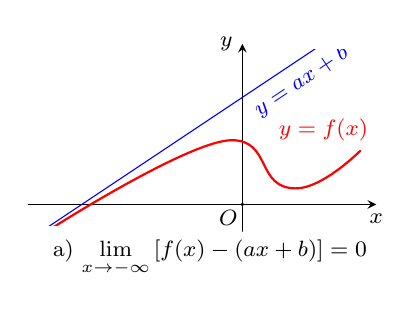
\begin{tikzpicture}[scale=0.68,>=stealth, font=\footnotesize, line join=round, line cap=round]
			\def\xmin{-4} \def\xmax{2.5}
			\def\ymin{-0.5} \def\ymax{3}
			%\draw[color=gray!50,dashed] (\xmin,\ymin) grid (\xmax,\ymax);
			\draw[->] (\xmin,0)--(\xmax,0) node [below]{$x$};
			\draw[->] (0,\ymin)--(0,\ymax) node [left]{$y$};
			\fill (0,0) circle (1pt) node[shift={(-135:2.5mm)}]{$O$};
			\node at (current bounding box.south) [below=-2pt] {a) $\lim\limits_{x \rightarrow-\infty}\left[f(x)-(ax+b)\right]=0$};
			\clip (\xmin+0.1,\ymin+0.1) rectangle (\xmax-0.1,\ymax-0.1);
			\draw[red,thick,smooth,samples=300,domain=\xmin:\xmax]
			(-3.8,-0.6)..controls +(34:0.5) and +(180:.75)
			..(-0.2,1.2)..controls +(0:0.75) and +(180:.75)
			..(1,0.3)..controls +(0:0.5) and +(80:0)
			..(2.2,1);
			\draw[blue,smooth,samples=300,domain=\xmin:\xmax] plot(\x,{2/3*(\x)+2});
			\path[blue] (-3,0)--(0,2)node[below,sloped,pos=1.3]{$y=ax+b$};
			\path[red] (0.5,1)node[above right]{$y=f(x)$};
		\end{tikzpicture}\hspace{2cm}
		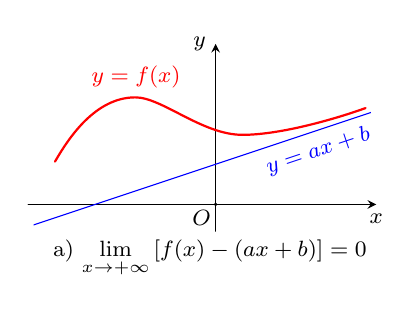
\begin{tikzpicture}[scale=0.68,>=stealth, font=\footnotesize, line join=round, line cap=round]
			\def\xmin{-3.5} \def\xmax{3}
			\def\ymin{-0.5} \def\ymax{3}
			%\draw[color=gray!50,dashed] (\xmin,\ymin) grid (\xmax,\ymax);
			\draw[->] (\xmin,0)--(\xmax,0) node [below]{$x$};
			\draw[->] (0,\ymin)--(0,\ymax) node [left]{$y$};
			\fill (0,0) circle (1pt) node[shift={(-135:2.5mm)}]{$O$};
			\node at (current bounding box.south) [below=-2pt] {a) $\lim\limits_{x \rightarrow+\infty}\left[f(x)-(ax+b)\right]=0$};
			\clip (\xmin+0.1,\ymin+0.1) rectangle (\xmax-0.1,\ymax-0.1);
			\draw[red,thick,smooth,samples=300,domain=\xmin:\xmax]
			(-3,0.8)..controls +(60:0.5) and +(180:.75)
			..(-1.5,2)..controls +(0:.5) and +(180:.75)
			..(0.5,1.3)..controls +(0:.75) and +(-160:.5)
			..(2.8,1.8);
			\draw[blue,smooth,samples=300,domain=\xmin:\xmax] plot(\x,{1/3*(\x)+0.75});
			\path[blue] (-3,-0.25)--(0,0.75)node[below,sloped,pos=1.6]{$y=ax+b$};
			\path[red] (-2.5,2)node[above right]{$y=f(x)$};
		\end{tikzpicture}
	\end{center}		
	\item \indam{Các bước tìm TCX y = ax + b:}
	Ta xác định hệ số của $a$ và $b$ trong 2 trường hợp sau:
	\begin{boxdn}
		\begin{itemize}
			\item [\ding{172}] Tính $a=\lim\limits_{x \rightarrow+\infty} \dfrac{f(x)}{x}$, $b=\lim\limits_{x \rightarrow+\infty}[f(x)-ax]$.
			\item [\ding{173}] Tính $a=\lim\limits_{x \rightarrow-\infty} \dfrac{f(x)}{x}$, $b=\lim\limits_{x \rightarrow-\infty}[f(x)-ax]$.
		\end{itemize}
	\end{boxdn}
\end{enumerate}
